\newpage
\section{GUI Elementklassen}
\subsection{Interaktion des Clients mit anderen Modulen}
\begin{itemize}
\item Die meisten GUI Klassen leiten von \emph{AbstractClientUser} ab und speichern daher eine Referenz auf eine Instanz von \emph{MPD::Client}
      Sie können daher Funktionen wie queue\_add() direkt aufrufen.
      AbstractClientUser zwingt die abgeleitenden Klassen folgende Funktionen zu implementieren: 
\begin{verbatim} 
   1) void on_client_update(mpd_idle event, MPD::NotifyData& data)
   2) void on_connection_change(bool server_changed, bool is_connected)
\end{verbatim}
   \begin{enumerate}
   \item Wird aufgerufen sobald der Listener ein Event festgestellt hat. Für jedes eingetretene Event wird on\_client\_update()    
   einmal aufgerufen. ,,event'' ist dabei eine Enumeration aller möglichen Events, die von libmpdclient 
   vorgegeben werden. (Siehe auch \href{``http://www.musicpd.org/doc/libmpdclient/idle\_8h.html#a3378f7a24c714d7cb1058232330d7a1c''}{``libmpdclient''})
   ,,data'' ist eine Referenz auf eine Instanz von MPD::NotifyData. Die benutzenden Klassen können folgenden Funktionen so
   bei Events sofort die aktuellen Änderungen auslesen:
   \begin{itemize} 
     \item get\_status() gibt den aktuellen MPD::Status
     \item get\_song() gibt den aktuellen MPD::Song
     \item get\_statistics() gibt die aktuellen MPD::Statistics
   \end{itemize} 
   \item Wird vom Client aufgerufen sobald die Verbindung verloren geht.
         Dabei zeigt der übergebene boolean Wert ,,is\_connected'' an ob man connected oder disconnected wurde.
         ,,server\_changed'' soll dann anzeigen ob der Server derselbe ist wie beim zuvor geschehenen Connectvorgang.
         Dies ist beim ersten Start stets wahr. ,,server\_changed'' kann nicht wahr sein wenn ,,is\_connected'' falsch ist.
   \end{enumerate}
\item Ableitung von den oben beschriebenen abstrakten Klassen AbstractItemlist und AbstractFilebrowser, um alle Funktionen von AbstractItemGenerator nutzen zu können. Beispiele dazu folgen weiter unten.
\end{itemize}


\subsection{Hauptklassen}
Der GManager Namespace enthält Klassen die der Verwaltung und Kontrolle des Hauptfensters von Freya dienen,
jedoch nicht den eigentlichen Inhalt des Hauptfensters bereitstellen (dies soll von den Browserklassen getan werden)
Alle Klassen gehören nach dem MVC Paradigma der Controllerschicht an.
\\
Der Begriff ,,Browser'' wird im folgenden für die einzelnen Tabs benutzt die Links in der Sidebar zu finden sind. 
Beispiele dafür sind ,,Queue'', ,,Database'' und ,,Settings''.
\\
Viele Klassen sind nur stichpunktartig erklärt da sie oft einander ähnlich sind, und ein gewisser Freiraum bei der Implementierung der
GUI gelassen werden soll.

\newpage
\begin{figure}[htb!]
\subsubsection{AbstractBrowser}
	\centering
        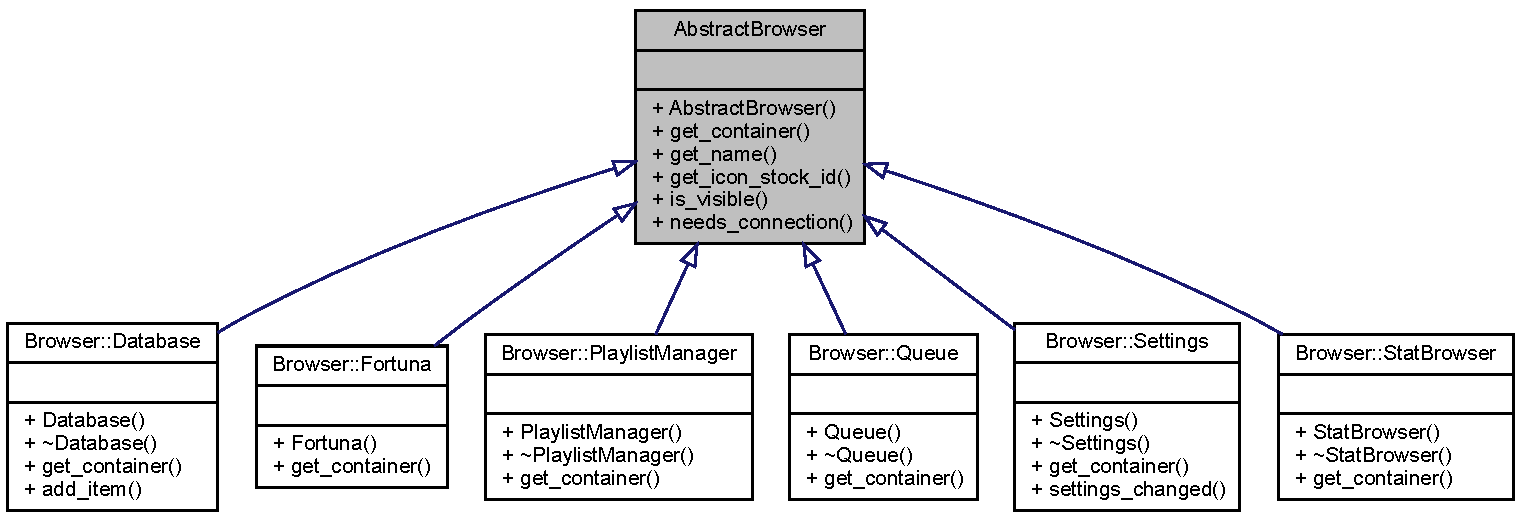
\includegraphics[width=\textwidth]{./gfx/class/abstractbrowser}
	\caption{Klassendiagramm zu AbstractBrowser}
	\label{g_abstract_browser}
\end{figure}


Eine abstrakte Basisklasse \ref{g_abstract_browser} durch die...
\begin{verbatim}
  Gtk::Widget * get_container(void) 
\end{verbatim}
..implementiert werden muss. Diese sollte den umliegenden Container des Browser als Pointer zurückgeben,
so dass \textit{GManager::BrowserList} diesen (und damit seine Kinder) im Hauptbereich anzeigen kann.
Siehe auch GManager::BrowserList für die nähere Erklärung zu den anderen nicht-abstrakten Methoden dieser Klasse.

\subsubsection{BrowserList}
%
%
% Ein Klassen (oder heiß das jetzt Kollab? :P) - diagramm zum hinzufügen eines Browsers
%
Zeigt eine Liste von Browsern in der Sidebar.
\begin{itemize} 
\item Bietet eine add() Methode die eine Referenz auf AbstractBrowser erwartet und fügt diesen Browser in der Sidebar hinzu.
\item set() zeigt den Browser im Hauptbereich, ohne ihn hinzuzufügen.
\end{itemize}
Die Klasse benutzt alle Methoden von AbstractBrowser um diesen entsprechend anzuzeigen:
\\
Der Container der im Hauptbereich beim Wechseln angezeigt wird
\begin{verbatim}
  Gtk::Widget * get_container();
\end{verbatim}
Welcher Name soll in der Sidebar angezeigt werden?
\begin{verbatim}
  Glib::ustring get_name();
\end{verbatim}
Welche Gtk::Stock::ID (eine ID die ein Icon repräsentiert) soll in der Liste angezeigt werden?
\begin{verbatim}
  Gtk::Stock::ID get_icon_stock_id();
\end{verbatim} 
Ist sichtbar in der Leiste?
\begin{verbatim}
  bool is_visible(); 
\end{verbatim}
Benötigt dieser Browser eine Verbindung zum funktionieren?
\begin{verbatim}
  bool needs_connection(); 
\end{verbatim}

Als \emph{View} wird ein Gtk::TreeView benutzt, die Browserreferenzen werden in einem Gtk::ListStore gespeichert,
was damit das Model darstellt. 

\subsubsection{Heartbeat}
%
% Falls Zeit ist hier noch ein simples Sequenzdiagramm
%
%
Diese Klasse soll alle 500ms ein Signal aussenden, die bisher vergangene Zeit summieren, und sich regelmäßig mit dem 
Client synchronisieren, so dass die summierte Zeit der aktuellen Zeit innerhalb des aktuellen Songs entspricht.
Über signal\_client\_update() können sich andere Klassen als Klienten registrieren:
\begin{verbatim}
  Heartbeat.signal_client_update().connect(<funktionspointer>);
\end{verbatim}
Der angegebene Funktionspointer wird dann aufgerufen und muss folgender Signatur entsprechen:
\begin{verbatim}
  void func(double time)
  {
      ...
  }
\end{verbatim}

Der übergebene Parameter ist die Zeit, die seit dem Instanzieren vergangen ist. 
Sie kann durch folgende Funktionen verändert werden:
\begin{verbatim}
void pause(void)  - Setzt das Zählen aus
void play(void)   - Fängt damit wieder an
void reset(void)  - Fängt von 0 wieder an
void get(void)    - Bekommt die jetzige Zeit
void set(void)    - Setzt die jetzige Zeit absolut und zählt von dort weiter
\end{verbatim}

Zusätzlich stoppt die Heartbeat Klasse das Zählen wenn der Client das Playback pausiert.
Wird es fortgesetzt, so wird play() aufgerufen. 
Zusätzlich wird bei jedem ,,Client Event'' der Zähler an der vergangen Zeit, im gerade spielenden Song, justiert.

\subsubsection{MenuList}
Kontrolliert und verwaltet die Anzeige (Sensitivität) und Steuerung der Menüleiste.

\subsubsection{NotifyManager}
Kontrolliert und verwaltet die Anzeige von Notifications bei entsprechenden ,,events''.
Greift dabei auf die Notifylib zurück.

\subsubsection{PlaybackButtons}
Kontrolliert die Anzeige der oberen rechten ,,Playbackbuttons'' Stop, Play/Pause, Next, Previous
Das Icon des Playbuttons wird entsprechend geändert falls das Playback pausiert ist,
bzw. fortgesetzt wird. Es sollen die Buttons \it Stop, Play/Pause, Previous und Next \rm angezeigt wird.

\subsubsection{Statusbar}
Kontrolliert die Anzeige der Statusbar (was den Text mit einfasst). 
Benutzt GManager::Heartbeat um die Zeitanzeige zu aktualisieren. Ansonsten bekommt es alle Informationen rein vom Client update.

\subsubsection{StatusIcons}
Kontrolliert und verwaltet Anzeige der Icons unter der Sidebar.
Bei Aktivierung sollen die Icons eingedrückt sein.
Folgende Icons sollen dargestellt werden:
\begin{itemize}
\item Repeat-Mode (Wiederholt Queue)
\item Consume-Mode (Entfernt Song nach Abspielen aus der Queue)
\item Random-Mode (Zufälliges Abspielen innerhalb der Queue)
\item Single-Mode (Hält nach Abspielen eines Songs an)
\end{itemize}

\subsubsection{Timeslider}
Zeigt und kontrolliert die aktuelle Zeit innerhalb des momentan spielenden Liedes.
Beim Klicken innerhalb der Timeline wird zur entsprechenden Stelle im Song gesprungen.
Benutzt GManager::Heartbeat um die Zeitanzeige zu aktualisieren.

\subsubsection{TitleLabel}
Verwaltet und kontrolliert Anzeige des Titels bzw. Künstlers und Albums in der Titelleiste sowie der ,,Next Song'' Anzeige in der Sidebar.

\subsubsection{Trayicon}
Verwaltet und kontrolliert Anzeige und Interaktion des Trayicons das optional angezeigt werden kann.
Dazu gehört auch die Definition und Anzeige des Popupmenüs, weshalb die Klasse von \textit{Browser::BasePopup} ableitet.
(Siehe dazu die Erklärung zu Browser::BasePopup weiter unten)

\subsubsection{Volumebutton}
Verwaltet und kontrolliert die Anzeige des Volumebuttons. Aus Performance Gründen sollen nur alle 0.05 Sekunden Volumeänderungen erlaubt werden.

\subsubsection{Window}
Verwaltet das Hauptfenster von Freya.
Falls das Verstecken des Fensters beim Schließen gewünscht ist (\emph{,,settings.trayicon.totrayonclose''} ist gesetzt),
so wird \emph{Gtk::Window::hide()} aufgerufen.
Andernfalls wird einfach der Mainloop beendet wodurch die Kontrolle zur main() Methode zurückkehrt.
Zudem wird eine get\_window() Methode bereitgestellt die das darunterliegende Fenster (ein Gtk::Window) zurückgibt.
Der Mainloop z.B. benötigt das als Startargument.
\section{Avahi Serverliste}
\subsubsection{Brower}

Die Avahi Klassen \emph{Avahi::Browser} und \emph{Avahi::View} gehören nach dem MVC Paradigma zur Controller und View Schicht. Bei
dieser Komponente wurde die Trennung zwischen Controller und View manuell durchgeführt.
\\
\\
Die Controller Klasse realisiert die technische Implementierung\footnote{http://de.wikipedia.org/wiki/Zeroconf} des ,,Avahi Browsers'' um MPD Server im Netzwerk zu finden.
\\
\\
Der View Part ist vom Controller völlig abgetrennt und dient lediglich zur Visualisierung der im Netzwerk gefundenen
MPD Server mit der Möglichkeit diese direkt auszuwählen.
\\
\\
Nach dem Start des Bowsers über den ,,Show List'' Button in den Freya Settings bekommt der Benutzer eine Liste mit sich im
gleichen Netzwerk befindenden MPD Servern aus welche der Benutzer direkt einen auswählen kann. Wurden keine MPD Server
gefunden oder läuft der Avahi Daemon nicht so bekommt der User einen entsprechenden Hinweis.
\\
\\
Um den Avahi-Dienst überhaupt betreiben zu können muss ein Avahi Daemon auf den jeweiligen
Systemen installiert sein und auch laufen. Außerdem müssen in der MPD Konfiguration die beiden Einträge ,,zeroconf\_enabled'' und ,,zeroconf\_name''
eingepflegt sein damit sich der MPD Server am Avahi Daemon registriert. Avahi muss dabei vor dem MPD Server gestartet werden.

Informationen zu Avahi selbst:
\begin{itemize}
\item \url{http://avahi.org/}
\end{itemize}

Informationen zur Programmierschnittstelle von Avahi:
\begin{itemize}
\item \url{http://avahi.org/download/doxygen/}
\end{itemize}

\paragraph{Browser:}
Er sollte mindestens folgende Schnittstellen bieten:
\begin{verbatim}
   Gtk::Window& get_window(void);
   bool is_connected(void);

   typedef sigc::signal<void,ustring,ustring,ustring,int> SelectNotify;
   SelectNotify& signal_selection_done(void);
\end{verbatim}
\begin{itemize}
\item get\_window() gibt das Dialogfenster der View zurück. (Zur Anzeige nötig)
\item is\_connected() zeigt durch 'true' an ob eine Verbindung zum Avahidaemon besteht
\item signal\_selection\_done() wird ausgelöst sobald der User in der View einen Server auswählt. 
      Da es sich hier wieder um ein sigc::signal handelt kann der Anwender sigc::signal::connect() anwenden.
      Der Prototyp der dabei übergeben wurden muss sieht wie folgt aus:
      \begin{verbatim}
      void (ustring ip, ustring hostname, ustring name, int port)
      {
        ...
      }
      \end{verbatim}
\end{itemize}

\paragraph{View:}
Die View stellt lediglich die Daten dar und bietet daher auch nur Möglichkeiten um Server zur Liste hinzuzufügen
und daraus zu löschen. Sie leitet von Gtk::Window ab, und wird daher nur über die Methoden von Gtk::Window angesprochen.
\begin{verbatim}
   void server_append(ip, hostname, name, port);
   void server_delete(name);
\end{verbatim}
